
\section{Clustering}\label{sec:evaluation-clustering}
Though the clustering stage of this detection scheme is to be used in realtime, this thesis research mostly consists of offline testing and evaluation. In the context of this thesis, an optimal outcome for the clustering stage would include clear distinction of clusters that reflect a differentiation between users. By using solely mouse data from the user, and generating features from this data, differentiating users through unlabeled data is the intended outcome in this evaluation.

A statistical software, JMP, was used to perform principal component analysis and generate clusters. Although there were multiple clustering methods available, all of which showed promising results, kmeans was the clustering method used in this research. Outputted distance and membership metrics reflect the level of effectiveness between different features used with the kmeans method. Since there were 10 users in the inputted dataset~\cite{balabit_dataset}, and the intention is to differentiate all users, the \textit{k} value was set to 10 in all clustering samples.

\begin{table}[h!]
	\centering
	\begin{tabular}{|c|c|c|c|c|c|c|c|c|}
		\hline
		\textbf{feature} & \textbf{PC1} & \textbf{PC2} & \textbf{PC3} & \textbf{PC4} & \textbf{PC5} & \textbf{PC6} & \textbf{PC7} & \textbf{sum} \\
		\hline
		vel-median & 0.07 & 0.29 & -0.09 & -0.02 & 0.04 & 0.07 & 0.06 & \textbf{43.72} \\
		vel-iqr & 0.08 & 0.19 & -0.28 & -0.09 & 0.05 & 0.21 & 0.18 & \textbf{35.59} \\
		yvel-median & 0.07 & 0.28 & 0.04 & 0.07 & 0.06 & -0.01 & 0.19 & \textbf{70.60} \\
		yvel-mode & 0.01 & 0.07 & -0.03 & 0.05 & -0.03 & -0.01 & 0.28 & \textbf{33.75} \\
		yvel-iqr & 0.08 & 0.22 & -0.12 & 0.01 & 0.12 & 0.18 & 0.30 & \textbf{78.26} \\
		accl-median & 0.06 & 0.31 & 0.07 & -0.01 & 0.07 & -0.02 & -0.13 & \textbf{35.89} \\
		theta-mean & 0.01 & 0.02 & 0.30 & 0.19 & 0.23 & 0.16 & 0.38 & \textbf{128.40} \\
		theta-median & 0.01 & 0.03 & 0.28 & 0.20 & 0.20 & 0.14 & 0.40 & \textbf{126.28} \\
		theta-iqr & -0.03 & -0.07 & 0.28 & 0.00 & 0.30 & 0.29 & -0.07 & \textbf{69.52} \\
		theta-stdev & -0.04 & -0.07 & 0.30 & 0.00 & 0.27 & 0.24 & -0.18 & \textbf{52.62} \\
		\hline
	\end{tabular}
	\caption{Results from PCA (all)}
	{\small Shown are the 8 features used as a result of the principal component analysis on all 48 features. Per the right-most sums column, the left-most column contains features that account for most of the variation of the data. Note how the theta features have such high values, despite them having the lowest original values. This may be a result of data standardization in JMP}
	\label{tab:pca-all-results}
\end{table}

By observing the plotted eigen vectors, the number of components chosen from PCA was the number of components needed to cumulatively attribute to at least 80\% of the variance in the inputted features. In the PCA that observes all 48 features, 7 components were needed to satisfy this 80\% threshold. Eigen vectors of each feature were summed and compared. The max sum of all features up to the nth component indicates that feature as having the most "weight" or influence on the variation in the data. A challenging aspect of PCA was deciding how many components to sum to. 7 components were chosen here. But that is only because 7 components were needed to satisfy a self-suggested threshold of 80\% that seemed reasonable. There is a need to analyze further to reinforce this approach.

\begin{table}[h!]
	\centering
	\begin{tabular}{|c|c|c|c|c|c|c|c|c|}
		\hline
		\textbf{PrinComp} & \textbf{01} & \textbf{02} & \textbf{03} & \textbf{04} & \textbf{05} & \textbf{06} & \textbf{07} & \textbf{08} \\
		\hline
		Eigen & 14.47 & 8.94 & 3.76 & 3.09 & 2.71 & 2.00 & 1.91 & 1.22 \\
		Per & 30.8 & 19.0 & 8.0 & 6.6 & 5.8 & 4.3 & 4.1 & 2.6 \\
		Cum & 30.1 & 49.8 & 57.8 & 64.4 & 70.2 & 74.4 & 78.5 & 81.1 \\
		\hline
	\end{tabular}
	\caption{Eigen values in PCA (all)}
	{\small Principal component analysis on all 48 features}
	\label{tab:eigen-values-all}
\end{table}

% COMMENT BEGIN
\iffalse
\begin{table}[h!]
	\centering
	\begin{tabular}{|c|c|c|c|c|c|c|}
		\hline
		\textbf{feature} & \textbf{Prin1} & \textbf{Prin2} & \textbf{Prin3} & \textbf{Prin4} & \textbf{Prin5} & \textbf{sum} \\
		\hline
		vel-mean & 0.22 & -0.06 & 0.21 & -0.02 & -0.09 & 26.25 \\
		\textbf{vel-median} & \textbf{0.07} & \textbf{0.30} & \textbf{0.08} & \textbf{-0.03} & \textbf{0.09} & \textbf{50.47} \\
		\textbf{vel-mode} & \textbf{0.03} & \textbf{0.01} & \textbf{0.14} & \textbf{-0.07} & \textbf{0.41} & \textbf{51.17} \\
		\textbf{vel-iqr} & \textbf{0.08} & \textbf{0.21} & \textbf{0.20} & \textbf{-0.12} & \textbf{0.35} & \textbf{71.79} \\
		vel-stdev & 0.24 & -0.09 & 0.14 & -0.02 & -0.09 & 18.35 \\
		\textbf{vel-min} & \textbf{0.00} & \textbf{0.04} & \textbf{0.16} & \textbf{0.53} & \textbf{0.03} & \textbf{75.72} \\
		vel-max & 0.24 & -0.09 & 0.00 & -0.02 & -0.02 & 11.43 \\
		vel-range & 0.24 & -0.09 & 0.00 & -0.02 & -0.02 & 11.43 \\
		xvel-mean & 0.22 & -0.06 & 0.21 & -0.02 & -0.09 & 26.43 \\
		xvel-median & 0.07 & 0.29 & 0.07 & -0.03 & 0.06 & 45.72 \\
		xvel-mode & 0.02 & 0.05 & 0.09 & -0.01 & 0.28 & 42.32 \\
		\textbf{xvel-iqr} & \textbf{0.08} & \textbf{0.21} & \textbf{0.19} & \textbf{-0.12} & \textbf{0.31} & \textbf{66.92} \\
		xvel-stdev & 0.24 & -0.09 & 0.14 & -0.02 & -0.08 & 18.35 \\
		\textbf{xvel-min} & \textbf{-0.01} & \textbf{0.03} & \textbf{0.14} & \textbf{0.51} & \textbf{0.00} & \textbf{68.50} \\
		xvel-max & 0.24 & -0.09 & 0.00 & -0.02 & -0.02 & 11.39 \\
		xvel-range & 0.24 & -0.09 & 0.00 & -0.02 & -0.02 & 11.39 \\
		yvel-mean & 0.22 & -0.06 & 0.21 & -0.02 & -0.10 & 25.13 \\
		yvel-median & 0.06 & 0.28 & 0.02 & 0.00 & -0.01 & 35.57 \\
		yvel-mode & 0.01 & 0.07 & 0.05 & 0.00 & 0.16 & 28.91 \\
		\textbf{yvel-iqr} & \textbf{0.08} & \textbf{0.23} & \textbf{0.16} & \textbf{-0.09} & \textbf{0.24} & \textbf{61.37} \\
		yvel-stdev & 0.24 & -0.09 & 0.14 & -0.02 & -0.09 & 18.32 \\
		\textbf{yvel-min} & \textbf{0.00} & \textbf{0.03} & \textbf{0.15} & \textbf{0.48} & \textbf{0.02} & \textbf{68.27} \\
		yvel-max & 0.24 & -0.09 & 0.00 & -0.02 & -0.02 & 11.44 \\
		yvel-range & 0.24 & -0.09 & 0.00 & -0.02 & -0.02 & 11.44 \\
		accl-mean & 0.22 & 0.04 & 0.08 & 0.01 & -0.07 & 27.59 \\
		accl-median & 0.06 & 0.31 & -0.04 & 0.01 & -0.15 & 19.17 \\
		accl-mode & 0.03 & 0.16 & 0.05 & -0.03 & 0.02 & 23.17 \\
		accl-iqr & 0.06 & 0.31 & -0.03 & -0.01 & -0.12 & 22.41 \\
		accl-stdev & 0.24 & -0.05 & -0.03 & 0.03 & 0.03 & 20.82 \\
		accl-min & 0.00 & -0.02 & 0.11 & 0.30 & 0.08 & 46.13 \\
		accl-max & 0.21 & -0.03 & -0.28 & 0.08 & 0.16 & 13.86 \\
		accl-range & 0.21 & -0.03 & -0.28 & 0.08 & 0.16 & 13.86 \\
		jerk-mean & 0.14 & 0.23 & -0.11 & 0.04 & -0.19 & 11.75 \\
		jerk-median & 0.05 & 0.30 & -0.09 & 0.02 & -0.24 & 4.40 \\
		jerk-mode & 0.04 & 0.24 & -0.06 & 0.01 & -0.21 & 1.37 \\
		jerk-iqr & 0.05 & 0.30 & -0.09 & 0.02 & -0.24 & 3.14 \\
		jerk-stdev & 0.19 & 0.04 & -0.26 & 0.09 & 0.09 & 15.33 \\
		jerk-min & 0.00 & 0.01 & 0.06 & 0.18 & 0.04 & 29.47 \\
		jerk-max & 0.14 & 0.03 & -0.40 & 0.12 & 0.21 & 9.23 \\
		jerk-range & 0.14 & 0.03 & -0.40 & 0.12 & 0.21 & 9.23 \\
		\hline
	\end{tabular}
	\caption{Results from PCA (without theta)}
	{\small \textbf{Shown is a complete list} of the features used in the principal component analysis. Note that the theta features are not used in the PCA. The selected features used as a result of the PCA are in bold}
	\label{tab:pca-without-theta-results}
\end{table}

\begin{table}[h!]
	\centering
	\begin{tabular}{|c|c|c|c|c|c|c|}
		\hline
		\textbf{PrinComp} & \textbf{01} & \textbf{02} & \textbf{03} & \textbf{04} & \textbf{05} & \textbf{06} \\
		\hline
		Eigen & 14.43 & 8.67 & 3.28 & 2.57 & 2.11 & 1.21 \\
		Per & 36.1 & 21.7 & 8.2 & 6.4 & 5.3 & 3.0 \\
		Cum & 36.1 & 57.7 & 65.9 & 72.4 & 77.6 & 80.7 \\
		\hline
	\end{tabular}
	\caption{Eigen values in PCA (without theta)}
	{\small Due to the "all" PCA showing low relevance of the theta features, a corresponding PCA on the remaining 40 features was performed. Those results are show here}
	\label{tab:eigen-values-without-theta}
\end{table}
\fi
% COMMENT END

Once the principal components were chosen, the clustering stage begins. Note that the PCA step is not going to be a part of the detection scheme. The only reason why it was applied here was to see which mouse movement features are most effective in user differentiation by clustering. Despite the PCA-generated features, there were a number of clustering version used for comparison. The \textbf{mean}, \textbf{median}, \textbf{mode}, \textbf{standard deviation}, and the \textbf{interquartile range} of each of the 6 movement features, \textit{velocity}, \textit{horizontal velocity}, \textit{vertical velocity}, \textit{acceleration}, \textit{jerk}, and \textit{theta}, were used to build clusters. Of all 48 feature vectors that are to be used in clustering, 6 features, one movement feature per statistical value, were chosen as parameters to cluster.

\begin{table}[h!]
	\centering
	\begin{tabular}{ |c|c|c|c|c|c| }
		\hline
		\textbf{features{\_}set} & \textbf{pop{\_}stdev} & \textbf{pop{\_}range} & \textbf{bias} & \textbf{dist{\_}mean} & \textbf{dist{\_}stdev} \\
		\hline
		iqr & 152.42 & 14-445 & 3.628 & 1.794 & 2.012 \\
		mean & 294.60 & 1-732 & 2.647 & 2.037 & 1.846 \\
		median & 174.16 & 1-478 & 3.475 & 1.369 & 1.374 \\
		mode & 477.47 & 1-1523 & 2.360 & 2.480 & 3.073 \\
		stdev & 329.97 & 1-837 & 1.054 & 2.098 & 1.892 \\
		pca{\_}8 & 215.36 & 2-590 & 1.272 & 5.859 & 4.397 \\
		pca{\_}10 & 139.14 & 2-396 & 1.400 & 3.862 & 3.523 \\
		\hline
	\end{tabular}
	\caption{Clustering distribution results}
	\label{tab:clustering-distribution-results}
\end{table}

For example, the "mean" features set used as parameters for clustering were \textbf{velocity}-\textit{mean}, \textbf{horizontal velocity}-\textit{mean}, \textbf{vertical velocity}-\textit{mean}, \textbf{acceleration}-\textit{mean}, \textbf{jerk}-\textit{mean}, and \textbf{theta}-\textit{mean}. This pattern continued through all 6 of the movement features, over all 8 of the statistical features. Hence the 48 features to choose from.

\begin{figure}[h!]
	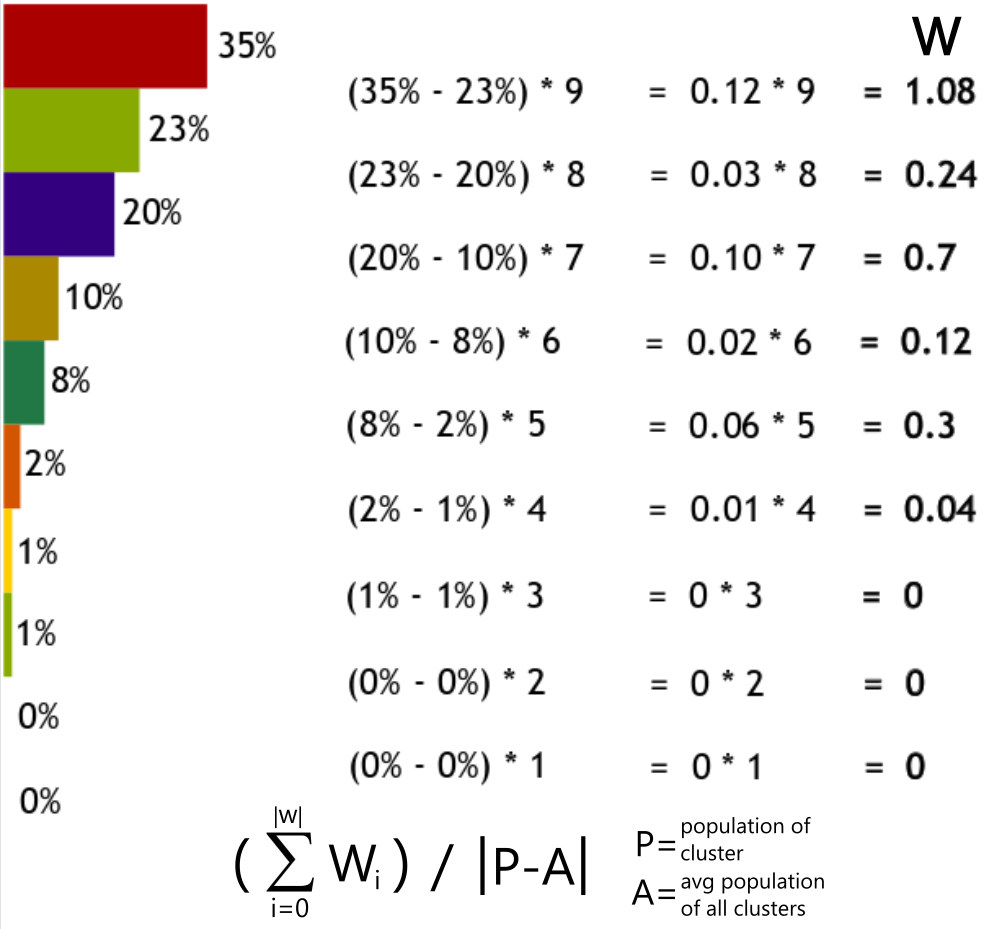
\includegraphics[width=.8\columnwidth]{figures/user_freq_distribution}

	\caption{User frequency bias metric}
	\label{fig:user_freq_bias_metric}
	{\small The user frequency bias metric describes the distribution of users in a cluster. A high value indicates that the cluster is biased to a certain user(s). A low value indicates that the cluster is not biased to any user(s) and is evenly spread. This metric accounts for variance and weights applied to the hierarchy of frequencies.}
\end{figure}

%
\begin{appendices}
\chapter{Clusters User Frequency Tables}\label{ch:clusers-user-frequency-tables}

\begin{table}
\centering
% cluster 2 of cluster_distances_iqr
\begin{tabular}{ |c|c|c|c| }
	\hline
	\textbf{user} & \textbf{freq} & \textbf{\%} & \textbf{wgt} \\
	\hline
	u15 & 70 & 20 & -- \\
	u16 & 67 & 19 & 0.1 \\
	u12 & 47 & 14 & 0.4 \\
	u35 & 39 & 11 & 0.1 \\
	u23 & 31 & 9 & 0.1 \\
	u7 & 24 & 7 & 0.1 \\
	u21 & 23 & 7 & 0.0 \\
	u9 & 21 & 6 & 0.0 \\
	u20 & 12 & 3 & 0.0 \\
	u29 & 10 & 3 & 0.0 \\
	 & 344 & & \textbf{0.5} \\
	\hline
\end{tabular}
% cluster 3 of cluster_distances_iqr
\begin{tabular}{ |c|c|c|c| }
	\hline
	\textbf{user} & \textbf{freq} & \textbf{\%} & \textbf{wgt} \\
	\hline
	u15 & 32 & 23 & -- \\
	u20 & 19 & 14 & 0.8 \\
	u35 & 17 & 12 & 0.1 \\
	u12 & 17 & 12 & 0.0 \\
	u16 & 16 & 12 & 0.0 \\
	u23 & 13 & 9 & 0.1 \\
	u21 & 8 & 6 & 0.1 \\
	u7 & 8 & 6 & 0.0 \\
	u9 & 6 & 4 & 0.0 \\
	u29 & 2 & 1 & 0.0 \\
	 & 138 & & \textbf{3.7} \\
	\hline
\end{tabular}
% cluster 6 of cluster_distances_iqr
\begin{tabular}{ |c|c|c|c| }
	\hline
	\textbf{user} & \textbf{freq} & \textbf{\%} & \textbf{wgt} \\
	\hline
	u29 & 61 & 18 & -- \\
	u35 & 52 & 15 & 0.2 \\
	u12 & 46 & 14 & 0.1 \\
	u15 & 45 & 13 & 0.0 \\
	u23 & 43 & 13 & 0.0 \\
	u16 & 27 & 8 & 0.2 \\
	u21 & 23 & 7 & 0.0 \\
	u9 & 14 & 4 & 0.1 \\
	u7 & 14 & 4 & 0.0 \\
	u20 & 13 & 4 & 0.0 \\
	 & 338 & & \textbf{0.4} \\
	\hline
\end{tabular}
% cluster 4 of cluster_distances_iqr
\begin{tabular}{ |c|c|c|c| }
	\hline
	\textbf{user} & \textbf{freq} & \textbf{\%} & \textbf{wgt} \\
	\hline
	u7 & 34 & 63 & -- \\
	u20 & 10 & 19 & 3.6 \\
	u12 & 3 & 6 & 0.9 \\
	u15 & 3 & 6 & 0.0 \\
	u23 & 2 & 4 & 0.1 \\
	u29 & 1 & 2 & 0.1 \\
	u16 & 1 & 2 & 0.0 \\
	u21 & 0 & 0 & 0.0 \\
	u9 & 0 & 0 & 0.0 \\
	u35 & 0 & 0 & 0.0 \\
	 & 54 & & \textbf{4.1} \\
	\hline
\end{tabular}
% cluster 10 of cluster_distances_iqr
\begin{tabular}{ |c|c|c|c| }
	\hline
	\textbf{user} & \textbf{freq} & \textbf{\%} & \textbf{wgt} \\
	\hline
	u9 & 43 & 68 & -- \\
	u20 & 12 & 19 & 3.9 \\
	u7 & 3 & 5 & 1.0 \\
	u23 & 2 & 3 & 0.1 \\
	u12 & 2 & 3 & 0.0 \\
	u15 & 1 & 2 & 0.1 \\
	u21 & 0 & 0 & 0.0 \\
	u35 & 0 & 0 & 0.0 \\
	u29 & 0 & 0 & 0.0 \\
	u16 & 0 & 0 & 0.0 \\
	 & 63 & & \textbf{4.9} \\
	\hline
\end{tabular}
% cluster 7 of cluster_distances_iqr
\begin{tabular}{ |c|c|c|c| }
	\hline
	\textbf{user} & \textbf{freq} & \textbf{\%} & \textbf{wgt} \\
	\hline
	u15 & 9 & 19 & -- \\
	u35 & 7 & 15 & 0.3 \\
	u9 & 5 & 10 & 0.3 \\
	u23 & 5 & 10 & 0.0 \\
	u12 & 5 & 10 & 0.0 \\
	u21 & 4 & 8 & 0.1 \\
	u7 & 4 & 8 & 0.0 \\
	u16 & 4 & 8 & 0.0 \\
	u29 & 3 & 6 & 0.0 \\
	u20 & 2 & 4 & 0.0 \\
	 & 48 & & \textbf{0.6} \\
	\hline
\end{tabular}
% cluster 8 of cluster_distances_iqr
\begin{tabular}{ |c|c|c|c| }
	\hline
	\textbf{user} & \textbf{freq} & \textbf{\%} & \textbf{wgt} \\
	\hline
	u7 & 39 & 55 & -- \\
	u20 & 18 & 25 & 2.4 \\
	u9 & 8 & 11 & 1.0 \\
	u29 & 2 & 3 & 0.5 \\
	u21 & 1 & 1 & 0.1 \\
	u35 & 1 & 1 & 0.0 \\
	u12 & 1 & 1 & 0.0 \\
	u15 & 1 & 1 & 0.0 \\
	u16 & 0 & 0 & 0.0 \\
	u23 & 0 & 0 & 0.0 \\
	 & 71 & & \textbf{4.1} \\
	\hline
\end{tabular}
% cluster 5 of cluster_distances_iqr
\begin{tabular}{ |c|c|c|c| }
	\hline
	\textbf{user} & \textbf{freq} & \textbf{\%} & \textbf{wgt} \\
	\hline
	u16 & 31 & 19 & -- \\
	u15 & 31 & 19 & 0.0 \\
	u12 & 26 & 16 & 0.2 \\
	u9 & 16 & 10 & 0.4 \\
	u21 & 15 & 9 & 0.0 \\
	u35 & 14 & 9 & 0.0 \\
	u29 & 11 & 7 & 0.1 \\
	u20 & 8 & 5 & 0.0 \\
	u23 & 6 & 4 & 0.0 \\
	u7 & 3 & 2 & 0.0 \\
	 & 161 & & \textbf{10.6} \\
	\hline
\end{tabular}
% cluster 1 of cluster_distances_iqr
\begin{tabular}{ |c|c|c|c| }
	\hline
	\textbf{user} & \textbf{freq} & \textbf{\%} & \textbf{wgt} \\
	\hline
	u12 & 93 & 21 & -- \\
	u35 & 62 & 14 & 0.6 \\
	u15 & 60 & 13 & 0.0 \\
	u16 & 55 & 12 & 0.1 \\
	u21 & 47 & 11 & 0.1 \\
	u23 & 40 & 9 & 0.1 \\
	u29 & 34 & 8 & 0.0 \\
	u7 & 19 & 4 & 0.1 \\
	u20 & 18 & 4 & 0.0 \\
	u9 & 17 & 4 & 0.0 \\
	 & 445 & & \textbf{0.4} \\
	\hline
\end{tabular}
\caption{User frequencies and bias metrics for (9 of 10) iqr clusters}
{\small The bias metric is in the bottom-right cell of each cluster table. The median bias metric for these clusters is 3.63}
\end{table}

\begin{table}
\centering
% cluster 2 of cluster_distances_mean
\begin{tabular}{ |c|c|c|c| }
	\hline
	\textbf{user} & \textbf{freq} & \textbf{\%} & \textbf{wgt} \\
	\hline
	u29 & 4 & 24 & -- \\
	u16 & 3 & 18 & 0.5 \\
	u12 & 3 & 18 & 0.0 \\
	u23 & 2 & 12 & 0.4 \\
	u21 & 1 & 6 & 0.3 \\
	u9 & 1 & 6 & 0.0 \\
	u35 & 1 & 6 & 0.0 \\
	u7 & 1 & 6 & 0.0 \\
	u15 & 1 & 6 & 0.0 \\
	u20 & 0 & 0 & 0.0 \\
	 & 17 & & \textbf{0.8} \\
	\hline
\end{tabular}
% cluster 3 of cluster_distances_mean
\begin{tabular}{ |c|c|c|c| }
	\hline
	\textbf{user} & \textbf{freq} & \textbf{\%} & \textbf{wgt} \\
	\hline
	u12 & 136 & 19 & -- \\
	u15 & 114 & 16 & 0.3 \\
	u16 & 106 & 15 & 0.1 \\
	u21 & 64 & 9 & 0.4 \\
	u23 & 59 & 8 & 0.0 \\
	u35 & 57 & 8 & 0.0 \\
	u20 & 51 & 7 & 0.0 \\
	u29 & 47 & 7 & 0.0 \\
	u9 & 39 & 6 & 0.0 \\
	u7 & 29 & 4 & 0.0 \\
	 & 702 & & \textbf{0.1} \\
	\hline
\end{tabular}
% cluster 6 of cluster_distances_mean
\begin{tabular}{ |c|c|c|c| }
	\hline
	\textbf{user} & \textbf{freq} & \textbf{\%} & \textbf{wgt} \\
	\hline
	u35 & 8 & 26 & -- \\
	u29 & 5 & 16 & 0.8 \\
	u15 & 5 & 16 & 0.0 \\
	u21 & 4 & 13 & 0.2 \\
	u7 & 3 & 10 & 0.2 \\
	u20 & 2 & 6 & 0.1 \\
	u12 & 2 & 6 & 0.0 \\
	u16 & 1 & 3 & 0.1 \\
	u23 & 1 & 3 & 0.0 \\
	u9 & 0 & 0 & 0.0 \\
	 & 31 & & \textbf{1.0} \\
	\hline
\end{tabular}
% cluster 4 of cluster_distances_mean
\begin{tabular}{ |c|c|c|c| }
	\hline
	\textbf{user} & \textbf{freq} & \textbf{\%} & \textbf{wgt} \\
	\hline
	u12 & 2 & 100 & -- \\
	u21 & 0 & 0 & 8.0 \\
	u9 & 0 & 0 & 0.0 \\
	u20 & 0 & 0 & 0.0 \\
	u35 & 0 & 0 & 0.0 \\
	u7 & 0 & 0 & 0.0 \\
	u29 & 0 & 0 & 0.0 \\
	u16 & 0 & 0 & 0.0 \\
	u23 & 0 & 0 & 0.0 \\
	u15 & 0 & 0 & 0.0 \\
	 & 2 & & \textbf{4.8} \\
	\hline
\end{tabular}
% cluster 10 of cluster_distances_mean
\begin{tabular}{ |c|c|c|c| }
	\hline
	\textbf{user} & \textbf{freq} & \textbf{\%} & \textbf{wgt} \\
	\hline
	u7 & 86 & 48 & -- \\
	u9 & 41 & 23 & 2.0 \\
	u20 & 30 & 17 & 0.4 \\
	u15 & 6 & 3 & 0.8 \\
	u12 & 5 & 3 & 0.0 \\
	u23 & 4 & 2 & 0.0 \\
	u29 & 3 & 2 & 0.0 \\
	u35 & 2 & 1 & 0.0 \\
	u21 & 1 & 1 & 0.0 \\
	u16 & 1 & 1 & 0.0 \\
	 & 179 & & \textbf{28.1} \\
	\hline
\end{tabular}
% cluster 7 of cluster_distances_mean
\begin{tabular}{ |c|c|c|c| }
	\hline
	\textbf{user} & \textbf{freq} & \textbf{\%} & \textbf{wgt} \\
	\hline
	u35 & 3 & 75 & -- \\
	u7 & 1 & 25 & 4.0 \\
	u21 & 0 & 0 & 1.8 \\
	u9 & 0 & 0 & 0.0 \\
	u20 & 0 & 0 & 0.0 \\
	u29 & 0 & 0 & 0.0 \\
	u16 & 0 & 0 & 0.0 \\
	u23 & 0 & 0 & 0.0 \\
	u12 & 0 & 0 & 0.0 \\
	u15 & 0 & 0 & 0.0 \\
	 & 4 & & \textbf{3.5} \\
	\hline
\end{tabular}
% cluster 5 of cluster_distances_mean
\begin{tabular}{ |c|c|c|c| }
	\hline
	\textbf{user} & \textbf{freq} & \textbf{\%} & \textbf{wgt} \\
	\hline
	u29 & 1 & 100 & -- \\
	u21 & 0 & 0 & 8.0 \\
	u9 & 0 & 0 & 0.0 \\
	u20 & 0 & 0 & 0.0 \\
	u35 & 0 & 0 & 0.0 \\
	u7 & 0 & 0 & 0.0 \\
	u16 & 0 & 0 & 0.0 \\
	u23 & 0 & 0 & 0.0 \\
	u12 & 0 & 0 & 0.0 \\
	u15 & 0 & 0 & 0.0 \\
	 & 1 & & \textbf{4.8} \\
	\hline
\end{tabular}
% cluster 1 of cluster_distances_mean
\begin{tabular}{ |c|c|c|c| }
	\hline
	\textbf{user} & \textbf{freq} & \textbf{\%} & \textbf{wgt} \\
	\hline
	u15 & 3 & 43 & -- \\
	u9 & 1 & 14 & 2.3 \\
	u20 & 1 & 14 & 0.0 \\
	u16 & 1 & 14 & 0.0 \\
	u12 & 1 & 14 & 0.0 \\
	u21 & 0 & 0 & 0.6 \\
	u35 & 0 & 0 & 0.0 \\
	u7 & 0 & 0 & 0.0 \\
	u29 & 0 & 0 & 0.0 \\
	u23 & 0 & 0 & 0.0 \\
	 & 7 & & \textbf{1.8} \\
	\hline
\end{tabular}
% cluster 9 of cluster_distances_mean
\begin{tabular}{ |c|c|c|c| }
	\hline
	\textbf{user} & \textbf{freq} & \textbf{\%} & \textbf{wgt} \\
	\hline
	u15 & 124 & 17 & -- \\
	u35 & 122 & 17 & 0.0 \\
	u12 & 91 & 12 & 0.3 \\
	u16 & 89 & 12 & 0.0 \\
	u23 & 76 & 10 & 0.1 \\
	u29 & 64 & 9 & 0.1 \\
	u21 & 50 & 7 & 0.1 \\
	u9 & 48 & 7 & 0.0 \\
	u7 & 38 & 5 & 0.0 \\
	u20 & 30 & 4 & 0.0 \\
	 & 732 & & \textbf{0.1} \\
	\hline
\end{tabular}
\caption{User frequencies and bias metrics for (9 of 10) mean clusters}
{\small The bias metric is in the bottom-right cell of each cluster table. The median bias metric for these clusters is 2.65}
\end{table}

\begin{table}
\centering
% cluster 2 of cluster_distances_median
\begin{tabular}{ |c|c|c|c| }
	\hline
	\textbf{user} & \textbf{freq} & \textbf{\%} & \textbf{wgt} \\
	\hline
	u16 & 69 & 23 & -- \\
	u15 & 59 & 20 & 0.3 \\
	u35 & 38 & 13 & 0.5 \\
	u12 & 27 & 9 & 0.2 \\
	u23 & 23 & 8 & 0.1 \\
	u21 & 19 & 6 & 0.1 \\
	u9 & 18 & 6 & 0.0 \\
	u20 & 15 & 5 & 0.0 \\
	u29 & 15 & 5 & 0.0 \\
	u7 & 13 & 4 & 0.0 \\
	 & 296 & & \textbf{0.9} \\
	\hline
\end{tabular}
% cluster 3 of cluster_distances_median
\begin{tabular}{ |c|c|c|c| }
	\hline
	\textbf{user} & \textbf{freq} & \textbf{\%} & \textbf{wgt} \\
	\hline
	u12 & 37 & 22 & -- \\
	u15 & 26 & 16 & 0.5 \\
	u20 & 19 & 11 & 0.3 \\
	u21 & 18 & 11 & 0.0 \\
	u16 & 18 & 11 & 0.0 \\
	u23 & 16 & 10 & 0.0 \\
	u35 & 11 & 7 & 0.1 \\
	u9 & 8 & 5 & 0.0 \\
	u29 & 8 & 5 & 0.0 \\
	u7 & 6 & 4 & 0.0 \\
	 & 167 & & \textbf{150.0} \\
	\hline
\end{tabular}
% cluster 6 of cluster_distances_median
\begin{tabular}{ |c|c|c|c| }
	\hline
	\textbf{user} & \textbf{freq} & \textbf{\%} & \textbf{wgt} \\
	\hline
	u35 & 84 & 20 & -- \\
	u15 & 67 & 16 & 0.3 \\
	u12 & 57 & 14 & 0.2 \\
	u29 & 51 & 12 & 0.1 \\
	u23 & 43 & 10 & 0.1 \\
	u16 & 35 & 8 & 0.1 \\
	u7 & 26 & 6 & 0.1 \\
	u21 & 24 & 6 & 0.0 \\
	u9 & 19 & 5 & 0.0 \\
	u20 & 15 & 4 & 0.0 \\
	 & 421 & & \textbf{0.4} \\
	\hline
\end{tabular}
% cluster 4 of cluster_distances_median
\begin{tabular}{ |c|c|c|c| }
	\hline
	\textbf{user} & \textbf{freq} & \textbf{\%} & \textbf{wgt} \\
	\hline
	u16 & 24 & 20 & -- \\
	u15 & 17 & 14 & 0.5 \\
	u12 & 14 & 11 & 0.2 \\
	u20 & 13 & 11 & 0.0 \\
	u9 & 12 & 10 & 0.0 \\
	u35 & 11 & 9 & 0.0 \\
	u23 & 11 & 9 & 0.0 \\
	u29 & 9 & 7 & 0.0 \\
	u21 & 7 & 6 & 0.0 \\
	u7 & 5 & 4 & 0.0 \\
	 & 123 & & \textbf{1.6} \\
	\hline
\end{tabular}
% cluster 7 of cluster_distances_median
\begin{tabular}{ |c|c|c|c| }
	\hline
	\textbf{user} & \textbf{freq} & \textbf{\%} & \textbf{wgt} \\
	\hline
	u7 & 8 & 47 & -- \\
	u20 & 4 & 24 & 1.9 \\
	u9 & 1 & 6 & 1.2 \\
	u35 & 1 & 6 & 0.0 \\
	u29 & 1 & 6 & 0.0 \\
	u23 & 1 & 6 & 0.0 \\
	u15 & 1 & 6 & 0.0 \\
	u21 & 0 & 0 & 0.1 \\
	u16 & 0 & 0 & 0.0 \\
	u12 & 0 & 0 & 0.0 \\
	 & 17 & & \textbf{2.1} \\
	\hline
\end{tabular}
% cluster 8 of cluster_distances_median
\begin{tabular}{ |c|c|c|c| }
	\hline
	\textbf{user} & \textbf{freq} & \textbf{\%} & \textbf{wgt} \\
	\hline
	u9 & 48 & 40 & -- \\
	u7 & 37 & 31 & 0.7 \\
	u20 & 22 & 18 & 0.9 \\
	u12 & 4 & 3 & 0.9 \\
	u15 & 4 & 3 & 0.0 \\
	u35 & 2 & 2 & 0.1 \\
	u23 & 2 & 2 & 0.0 \\
	u21 & 1 & 1 & 0.0 \\
	u29 & 1 & 1 & 0.0 \\
	u16 & 0 & 0 & 0.0 \\
	 & 121 & & \textbf{5.6} \\
	\hline
\end{tabular}
% cluster 5 of cluster_distances_median
\begin{tabular}{ |c|c|c|c| }
	\hline
	\textbf{user} & \textbf{freq} & \textbf{\%} & \textbf{wgt} \\
	\hline
	u12 & 99 & 21 & -- \\
	u15 & 77 & 16 & 0.4 \\
	u16 & 53 & 11 & 0.4 \\
	u21 & 52 & 11 & 0.0 \\
	u35 & 45 & 9 & 0.1 \\
	u23 & 45 & 9 & 0.0 \\
	u29 & 39 & 8 & 0.0 \\
	u20 & 24 & 5 & 0.1 \\
	u9 & 22 & 5 & 0.0 \\
	u7 & 22 & 5 & 0.0 \\
	 & 478 & & \textbf{0.3} \\
	\hline
\end{tabular}
% cluster 1 of cluster_distances_median
\begin{tabular}{ |c|c|c|c| }
	\hline
	\textbf{user} & \textbf{freq} & \textbf{\%} & \textbf{wgt} \\
	\hline
	u7 & 40 & 78 & -- \\
	u9 & 2 & 4 & 6.0 \\
	u20 & 2 & 4 & 0.0 \\
	u12 & 2 & 4 & 0.0 \\
	u15 & 2 & 4 & 0.0 \\
	u35 & 1 & 2 & 0.1 \\
	u16 & 1 & 2 & 0.0 \\
	u23 & 1 & 2 & 0.0 \\
	u21 & 0 & 0 & 0.0 \\
	u29 & 0 & 0 & 0.0 \\
	 & 51 & & \textbf{5.2} \\
	\hline
\end{tabular}
% cluster 9 of cluster_distances_median
\begin{tabular}{ |c|c|c|c| }
	\hline
	\textbf{user} & \textbf{freq} & \textbf{\%} & \textbf{wgt} \\
	\hline
	u16 & 1 & 100 & -- \\
	u21 & 0 & 0 & 8.0 \\
	u9 & 0 & 0 & 0.0 \\
	u20 & 0 & 0 & 0.0 \\
	u35 & 0 & 0 & 0.0 \\
	u7 & 0 & 0 & 0.0 \\
	u29 & 0 & 0 & 0.0 \\
	u23 & 0 & 0 & 0.0 \\
	u12 & 0 & 0 & 0.0 \\
	u15 & 0 & 0 & 0.0 \\
	 & 1 & & \textbf{4.8} \\
	\hline
\end{tabular}
\caption{User frequencies and bias metrics for (9 of 10) median clusters}
{\small The bias metric is in the bottom-right cell of each cluster table. The median bias metric for these clusters is 3.48}
\end{table}

\begin{table}
\centering
% cluster 3 of cluster_distances_mode
\begin{tabular}{ |c|c|c|c| }
	\hline
	\textbf{user} & \textbf{freq} & \textbf{\%} & \textbf{wgt} \\
	\hline
	u7 & 4 & 57 & -- \\
	u35 & 2 & 29 & 2.3 \\
	u12 & 1 & 14 & 1.0 \\
	u21 & 0 & 0 & 0.9 \\
	u9 & 0 & 0 & 0.0 \\
	u20 & 0 & 0 & 0.0 \\
	u29 & 0 & 0 & 0.0 \\
	u16 & 0 & 0 & 0.0 \\
	u23 & 0 & 0 & 0.0 \\
	u15 & 0 & 0 & 0.0 \\
	 & 7 & & \textbf{2.6} \\
	\hline
\end{tabular}
% cluster 6 of cluster_distances_mode
\begin{tabular}{ |c|c|c|c| }
	\hline
	\textbf{user} & \textbf{freq} & \textbf{\%} & \textbf{wgt} \\
	\hline
	u16 & 1 & 100 & -- \\
	u21 & 0 & 0 & 8.0 \\
	u9 & 0 & 0 & 0.0 \\
	u20 & 0 & 0 & 0.0 \\
	u35 & 0 & 0 & 0.0 \\
	u7 & 0 & 0 & 0.0 \\
	u29 & 0 & 0 & 0.0 \\
	u23 & 0 & 0 & 0.0 \\
	u12 & 0 & 0 & 0.0 \\
	u15 & 0 & 0 & 0.0 \\
	 & 1 & & \textbf{4.8} \\
	\hline
\end{tabular}
% cluster 4 of cluster_distances_mode
\begin{tabular}{ |c|c|c|c| }
	\hline
	\textbf{user} & \textbf{freq} & \textbf{\%} & \textbf{wgt} \\
	\hline
	u15 & 27 & 24 & -- \\
	u12 & 22 & 19 & 0.4 \\
	u16 & 17 & 15 & 0.3 \\
	u35 & 15 & 13 & 0.1 \\
	u7 & 8 & 7 & 0.3 \\
	u21 & 7 & 6 & 0.0 \\
	u9 & 7 & 6 & 0.0 \\
	u29 & 4 & 4 & 0.1 \\
	u23 & 4 & 4 & 0.0 \\
	u20 & 2 & 2 & 0.0 \\
	 & 113 & & \textbf{2.2} \\
	\hline
\end{tabular}
% cluster 10 of cluster_distances_mode
\begin{tabular}{ |c|c|c|c| }
	\hline
	\textbf{user} & \textbf{freq} & \textbf{\%} & \textbf{wgt} \\
	\hline
	u20 & 1 & 100 & -- \\
	u21 & 0 & 0 & 8.0 \\
	u9 & 0 & 0 & 0.0 \\
	u35 & 0 & 0 & 0.0 \\
	u7 & 0 & 0 & 0.0 \\
	u29 & 0 & 0 & 0.0 \\
	u16 & 0 & 0 & 0.0 \\
	u23 & 0 & 0 & 0.0 \\
	u12 & 0 & 0 & 0.0 \\
	u15 & 0 & 0 & 0.0 \\
	 & 1 & & \textbf{4.8} \\
	\hline
\end{tabular}
% cluster 7 of cluster_distances_mode
\begin{tabular}{ |c|c|c|c| }
	\hline
	\textbf{user} & \textbf{freq} & \textbf{\%} & \textbf{wgt} \\
	\hline
	u7 & 3 & 100 & -- \\
	u21 & 0 & 0 & 8.0 \\
	u9 & 0 & 0 & 0.0 \\
	u20 & 0 & 0 & 0.0 \\
	u35 & 0 & 0 & 0.0 \\
	u29 & 0 & 0 & 0.0 \\
	u16 & 0 & 0 & 0.0 \\
	u23 & 0 & 0 & 0.0 \\
	u12 & 0 & 0 & 0.0 \\
	u15 & 0 & 0 & 0.0 \\
	 & 3 & & \textbf{4.9} \\
	\hline
\end{tabular}
% cluster 8 of cluster_distances_mode
\begin{tabular}{ |c|c|c|c| }
	\hline
	\textbf{user} & \textbf{freq} & \textbf{\%} & \textbf{wgt} \\
	\hline
	u35 & 2 & 33 & -- \\
	u9 & 1 & 17 & 1.3 \\
	u20 & 1 & 17 & 0.0 \\
	u29 & 1 & 17 & 0.0 \\
	u16 & 1 & 17 & 0.0 \\
	u21 & 0 & 0 & 0.7 \\
	u7 & 0 & 0 & 0.0 \\
	u23 & 0 & 0 & 0.0 \\
	u12 & 0 & 0 & 0.0 \\
	u15 & 0 & 0 & 0.0 \\
	 & 6 & & \textbf{1.2} \\
	\hline
\end{tabular}
% cluster 5 of cluster_distances_mode
\begin{tabular}{ |c|c|c|c| }
	\hline
	\textbf{user} & \textbf{freq} & \textbf{\%} & \textbf{wgt} \\
	\hline
	u15 & 2 & 33 & -- \\
	u21 & 1 & 17 & 1.3 \\
	u29 & 1 & 17 & 0.0 \\
	u16 & 1 & 17 & 0.0 \\
	u23 & 1 & 17 & 0.0 \\
	u9 & 0 & 0 & 0.7 \\
	u20 & 0 & 0 & 0.0 \\
	u35 & 0 & 0 & 0.0 \\
	u7 & 0 & 0 & 0.0 \\
	u12 & 0 & 0 & 0.0 \\
	 & 6 & & \textbf{1.2} \\
	\hline
\end{tabular}
% cluster 1 of cluster_distances_mode
\begin{tabular}{ |c|c|c|c| }
	\hline
	\textbf{user} & \textbf{freq} & \textbf{\%} & \textbf{wgt} \\
	\hline
	u15 & 221 & 15 & -- \\
	u12 & 211 & 14 & 0.1 \\
	u16 & 180 & 12 & 0.1 \\
	u35 & 174 & 11 & 0.0 \\
	u7 & 141 & 9 & 0.1 \\
	u23 & 136 & 9 & 0.0 \\
	u9 & 122 & 8 & 0.0 \\
	u29 & 118 & 8 & 0.0 \\
	u21 & 111 & 7 & 0.0 \\
	u20 & 109 & 7 & 0.0 \\
	 & 1523 & & \textbf{0.0} \\
	\hline
\end{tabular}
% cluster 9 of cluster_distances_mode
\begin{tabular}{ |c|c|c|c| }
	\hline
	\textbf{user} & \textbf{freq} & \textbf{\%} & \textbf{wgt} \\
	\hline
	u12 & 6 & 40 & -- \\
	u21 & 2 & 13 & 2.1 \\
	u7 & 2 & 13 & 0.0 \\
	u15 & 2 & 13 & 0.0 \\
	u20 & 1 & 7 & 0.3 \\
	u16 & 1 & 7 & 0.0 \\
	u23 & 1 & 7 & 0.0 \\
	u9 & 0 & 0 & 0.1 \\
	u35 & 0 & 0 & 0.0 \\
	u29 & 0 & 0 & 0.0 \\
	 & 15 & & \textbf{1.6} \\
	\hline
\end{tabular}
\caption{User frequencies and bias metrics for (9 of 10) mode clusters}
{\small The bias metric is in the bottom-right cell of each cluster table. The median bias metric for these clusters is 2.36}
\end{table}

\begin{table}
\centering
% cluster 2 of cluster_distances_pca_top_8_without_theta
\begin{tabular}{ |c|c|c|c| }
	\hline
	\textbf{user} & \textbf{freq} & \textbf{\%} & \textbf{wgt} \\
	\hline
	u16 & 4 & 36 & -- \\
	u35 & 2 & 18 & 1.5 \\
	u15 & 2 & 18 & 0.0 \\
	u21 & 1 & 9 & 0.5 \\
	u7 & 1 & 9 & 0.0 \\
	u23 & 1 & 9 & 0.0 \\
	u9 & 0 & 0 & 0.3 \\
	u20 & 0 & 0 & 0.0 \\
	u29 & 0 & 0 & 0.0 \\
	u12 & 0 & 0 & 0.0 \\
	 & 11 & & \textbf{1.5} \\
	\hline
\end{tabular}
% cluster 3 of cluster_distances_pca_top_8_without_theta
\begin{tabular}{ |c|c|c|c| }
	\hline
	\textbf{user} & \textbf{freq} & \textbf{\%} & \textbf{wgt} \\
	\hline
	u15 & 17 & 16 & -- \\
	u16 & 16 & 15 & 0.1 \\
	u21 & 13 & 12 & 0.2 \\
	u35 & 13 & 12 & 0.0 \\
	u29 & 10 & 9 & 0.1 \\
	u20 & 9 & 8 & 0.0 \\
	u12 & 9 & 8 & 0.0 \\
	u7 & 8 & 7 & 0.0 \\
	u9 & 7 & 6 & 0.0 \\
	u23 & 7 & 6 & 0.0 \\
	 & 109 & & \textbf{0.7} \\
	\hline
\end{tabular}
% cluster 4 of cluster_distances_pca_top_8_without_theta
\begin{tabular}{ |c|c|c|c| }
	\hline
	\textbf{user} & \textbf{freq} & \textbf{\%} & \textbf{wgt} \\
	\hline
	u12 & 103 & 17 & -- \\
	u16 & 90 & 15 & 0.2 \\
	u15 & 84 & 14 & 0.1 \\
	u9 & 66 & 11 & 0.2 \\
	u35 & 57 & 10 & 0.1 \\
	u23 & 50 & 8 & 0.0 \\
	u21 & 36 & 6 & 0.1 \\
	u29 & 36 & 6 & 0.0 \\
	u20 & 35 & 6 & 0.0 \\
	u7 & 33 & 6 & 0.0 \\
	 & 590 & & \textbf{0.2} \\
	\hline
\end{tabular}
% cluster 10 of cluster_distances_pca_top_8_without_theta
\begin{tabular}{ |c|c|c|c| }
	\hline
	\textbf{user} & \textbf{freq} & \textbf{\%} & \textbf{wgt} \\
	\hline
	u7 & 5 & 26 & -- \\
	u15 & 4 & 21 & 0.4 \\
	u21 & 3 & 16 & 0.4 \\
	u20 & 3 & 16 & 0.0 \\
	u9 & 1 & 5 & 0.5 \\
	u35 & 1 & 5 & 0.0 \\
	u16 & 1 & 5 & 0.0 \\
	u12 & 1 & 5 & 0.0 \\
	u29 & 0 & 0 & 0.1 \\
	u23 & 0 & 0 & 0.0 \\
	 & 19 & & \textbf{0.9} \\
	\hline
\end{tabular}
% cluster 7 of cluster_distances_pca_top_8_without_theta
\begin{tabular}{ |c|c|c|c| }
	\hline
	\textbf{user} & \textbf{freq} & \textbf{\%} & \textbf{wgt} \\
	\hline
	u7 & 52 & 32 & -- \\
	u20 & 25 & 15 & 1.3 \\
	u15 & 19 & 12 & 0.3 \\
	u16 & 13 & 8 & 0.2 \\
	u9 & 12 & 7 & 0.0 \\
	u35 & 11 & 7 & 0.0 \\
	u23 & 10 & 6 & 0.0 \\
	u29 & 8 & 5 & 0.0 \\
	u12 & 8 & 5 & 0.0 \\
	u21 & 4 & 2 & 0.0 \\
	 & 162 & & \textbf{32.1} \\
	\hline
\end{tabular}
% cluster 8 of cluster_distances_pca_top_8_without_theta
\begin{tabular}{ |c|c|c|c| }
	\hline
	\textbf{user} & \textbf{freq} & \textbf{\%} & \textbf{wgt} \\
	\hline
	u35 & 85 & 16 & -- \\
	u12 & 85 & 16 & 0.0 \\
	u15 & 79 & 15 & 0.1 \\
	u23 & 62 & 12 & 0.2 \\
	u29 & 58 & 11 & 0.0 \\
	u21 & 46 & 9 & 0.1 \\
	u16 & 39 & 7 & 0.0 \\
	u20 & 31 & 6 & 0.0 \\
	u7 & 25 & 5 & 0.0 \\
	u9 & 23 & 4 & 0.0 \\
	 & 533 & & \textbf{0.1} \\
	\hline
\end{tabular}
% cluster 5 of cluster_distances_pca_top_8_without_theta
\begin{tabular}{ |c|c|c|c| }
	\hline
	\textbf{user} & \textbf{freq} & \textbf{\%} & \textbf{wgt} \\
	\hline
	u7 & 25 & 23 & -- \\
	u16 & 17 & 15 & 0.6 \\
	u15 & 15 & 14 & 0.1 \\
	u9 & 12 & 11 & 0.2 \\
	u35 & 8 & 7 & 0.2 \\
	u12 & 8 & 7 & 0.0 \\
	u21 & 7 & 6 & 0.0 \\
	u20 & 7 & 6 & 0.0 \\
	u29 & 6 & 5 & 0.0 \\
	u23 & 5 & 5 & 0.0 \\
	 & 110 & & \textbf{1.9} \\
	\hline
\end{tabular}
% cluster 1 of cluster_distances_pca_top_8_without_theta
\begin{tabular}{ |c|c|c|c| }
	\hline
	\textbf{user} & \textbf{freq} & \textbf{\%} & \textbf{wgt} \\
	\hline
	u15 & 5 & 29 & -- \\
	u16 & 4 & 24 & 0.5 \\
	u35 & 3 & 18 & 0.4 \\
	u20 & 2 & 12 & 0.4 \\
	u23 & 2 & 12 & 0.0 \\
	u29 & 1 & 6 & 0.2 \\
	u21 & 0 & 0 & 0.2 \\
	u9 & 0 & 0 & 0.0 \\
	u7 & 0 & 0 & 0.0 \\
	u12 & 0 & 0 & 0.0 \\
	 & 17 & & \textbf{1.1} \\
	\hline
\end{tabular}
% cluster 9 of cluster_distances_pca_top_8_without_theta
\begin{tabular}{ |c|c|c|c| }
	\hline
	\textbf{user} & \textbf{freq} & \textbf{\%} & \textbf{wgt} \\
	\hline
	u15 & 28 & 23 & -- \\
	u12 & 26 & 21 & 0.1 \\
	u16 & 17 & 14 & 0.5 \\
	u35 & 13 & 11 & 0.2 \\
	u21 & 10 & 8 & 0.1 \\
	u7 & 9 & 7 & 0.0 \\
	u9 & 8 & 7 & 0.0 \\
	u29 & 5 & 4 & 0.0 \\
	u23 & 5 & 4 & 0.0 \\
	u20 & 2 & 2 & 0.0 \\
	 & 123 & & \textbf{2.0} \\
	\hline
\end{tabular}
\caption{User frequencies and bias metrics for (9 of 10) pca top 8 without theta clusters}
{\small The bias metric is in the bottom-right cell of each cluster table. The median bias metric for these clusters is 1.27}
\end{table}

\begin{table}
\centering
% cluster 2 of cluster_distances_pca_top_10
\begin{tabular}{ |c|c|c|c| }
	\hline
	\textbf{user} & \textbf{freq} & \textbf{\%} & \textbf{wgt} \\
	\hline
	u15 & 65 & 23 & -- \\
	u16 & 51 & 18 & 0.4 \\
	u12 & 36 & 13 & 0.4 \\
	u35 & 27 & 10 & 0.2 \\
	u9 & 23 & 8 & 0.1 \\
	u23 & 19 & 7 & 0.1 \\
	u21 & 17 & 6 & 0.0 \\
	u20 & 15 & 5 & 0.0 \\
	u7 & 15 & 5 & 0.0 \\
	u29 & 9 & 3 & 0.0 \\
	 & 277 & & \textbf{1.1} \\
	\hline
\end{tabular}
% cluster 3 of cluster_distances_pca_top_10
\begin{tabular}{ |c|c|c|c| }
	\hline
	\textbf{user} & \textbf{freq} & \textbf{\%} & \textbf{wgt} \\
	\hline
	u20 & 18 & 23 & -- \\
	u12 & 15 & 19 & 0.3 \\
	u16 & 12 & 15 & 0.3 \\
	u23 & 10 & 13 & 0.2 \\
	u15 & 10 & 13 & 0.0 \\
	u21 & 4 & 5 & 0.3 \\
	u35 & 4 & 5 & 0.0 \\
	u7 & 3 & 4 & 0.0 \\
	u9 & 2 & 3 & 0.0 \\
	u29 & 0 & 0 & 0.0 \\
	 & 78 & & \textbf{1.2} \\
	\hline
\end{tabular}
% cluster 4 of cluster_distances_pca_top_10
\begin{tabular}{ |c|c|c|c| }
	\hline
	\textbf{user} & \textbf{freq} & \textbf{\%} & \textbf{wgt} \\
	\hline
	u9 & 43 & 65 & -- \\
	u7 & 6 & 9 & 4.5 \\
	u16 & 6 & 9 & 0.0 \\
	u15 & 4 & 6 & 0.2 \\
	u23 & 3 & 5 & 0.1 \\
	u20 & 1 & 2 & 0.1 \\
	u35 & 1 & 2 & 0.0 \\
	u29 & 1 & 2 & 0.0 \\
	u12 & 1 & 2 & 0.0 \\
	u21 & 0 & 0 & 0.0 \\
	 & 66 & & \textbf{4.8} \\
	\hline
\end{tabular}
% cluster 10 of cluster_distances_pca_top_10
\begin{tabular}{ |c|c|c|c| }
	\hline
	\textbf{user} & \textbf{freq} & \textbf{\%} & \textbf{wgt} \\
	\hline
	u12 & 88 & 22 & -- \\
	u21 & 52 & 13 & 0.7 \\
	u15 & 51 & 13 & 0.0 \\
	u35 & 41 & 10 & 0.2 \\
	u16 & 40 & 10 & 0.0 \\
	u23 & 39 & 10 & 0.0 \\
	u29 & 31 & 8 & 0.1 \\
	u20 & 21 & 5 & 0.1 \\
	u7 & 18 & 5 & 0.0 \\
	u9 & 15 & 4 & 0.0 \\
	 & 396 & & \textbf{0.5} \\
	\hline
\end{tabular}
% cluster 7 of cluster_distances_pca_top_10
\begin{tabular}{ |c|c|c|c| }
	\hline
	\textbf{user} & \textbf{freq} & \textbf{\%} & \textbf{wgt} \\
	\hline
	u20 & 2 & 40 & -- \\
	u9 & 1 & 20 & 1.6 \\
	u35 & 1 & 20 & 0.0 \\
	u16 & 1 & 20 & 0.0 \\
	u21 & 0 & 0 & 1.0 \\
	u7 & 0 & 0 & 0.0 \\
	u29 & 0 & 0 & 0.0 \\
	u23 & 0 & 0 & 0.0 \\
	u12 & 0 & 0 & 0.0 \\
	u15 & 0 & 0 & 0.0 \\
	 & 5 & & \textbf{1.6} \\
	\hline
\end{tabular}
% cluster 8 of cluster_distances_pca_top_10
\begin{tabular}{ |c|c|c|c| }
	\hline
	\textbf{user} & \textbf{freq} & \textbf{\%} & \textbf{wgt} \\
	\hline
	u16 & 53 & 18 & -- \\
	u15 & 51 & 17 & 0.1 \\
	u35 & 49 & 16 & 0.0 \\
	u12 & 33 & 11 & 0.3 \\
	u23 & 29 & 10 & 0.1 \\
	u9 & 20 & 7 & 0.1 \\
	u20 & 18 & 6 & 0.0 \\
	u21 & 17 & 6 & 0.0 \\
	u7 & 17 & 6 & 0.0 \\
	u29 & 15 & 5 & 0.0 \\
	 & 302 & & \textbf{0.4} \\
	\hline
\end{tabular}
% cluster 5 of cluster_distances_pca_top_10
\begin{tabular}{ |c|c|c|c| }
	\hline
	\textbf{user} & \textbf{freq} & \textbf{\%} & \textbf{wgt} \\
	\hline
	u7 & 80 & 66 & -- \\
	u20 & 25 & 20 & 3.6 \\
	u12 & 4 & 3 & 1.2 \\
	u15 & 4 & 3 & 0.0 \\
	u9 & 2 & 2 & 0.1 \\
	u35 & 2 & 2 & 0.0 \\
	u23 & 2 & 2 & 0.0 \\
	u21 & 1 & 1 & 0.0 \\
	u29 & 1 & 1 & 0.0 \\
	u16 & 1 & 1 & 0.0 \\
	 & 122 & & \textbf{10.7} \\
	\hline
\end{tabular}
% cluster 1 of cluster_distances_pca_top_10
\begin{tabular}{ |c|c|c|c| }
	\hline
	\textbf{user} & \textbf{freq} & \textbf{\%} & \textbf{wgt} \\
	\hline
	u29 & 58 & 20 & -- \\
	u35 & 52 & 18 & 0.2 \\
	u12 & 45 & 15 & 0.2 \\
	u15 & 42 & 14 & 0.1 \\
	u23 & 28 & 9 & 0.2 \\
	u16 & 21 & 7 & 0.1 \\
	u21 & 16 & 5 & 0.1 \\
	u9 & 13 & 4 & 0.0 \\
	u7 & 12 & 4 & 0.0 \\
	u20 & 9 & 3 & 0.0 \\
	 & 296 & & \textbf{0.7} \\
	\hline
\end{tabular}
% cluster 9 of cluster_distances_pca_top_10
\begin{tabular}{ |c|c|c|c| }
	\hline
	\textbf{user} & \textbf{freq} & \textbf{\%} & \textbf{wgt} \\
	\hline
	u15 & 26 & 20 & -- \\
	u12 & 18 & 14 & 0.5 \\
	u16 & 16 & 12 & 0.1 \\
	u35 & 15 & 11 & 0.0 \\
	u21 & 14 & 11 & 0.0 \\
	u23 & 12 & 9 & 0.1 \\
	u9 & 11 & 8 & 0.0 \\
	u29 & 8 & 6 & 0.0 \\
	u7 & 7 & 5 & 0.0 \\
	u20 & 5 & 4 & 0.0 \\
	 & 132 & & \textbf{2.0} \\
	\hline
\end{tabular}
\caption{User frequencies and bias metrics for (9 of 10) pca top 10 clusters}
{\small The bias metric is in the bottom-right cell of each cluster table. The median bias metric for these clusters is 1.4}
\end{table}

\begin{table}
\centering
% cluster 2 of cluster_distances_stdev
\begin{tabular}{ |c|c|c|c| }
	\hline
	\textbf{user} & \textbf{freq} & \textbf{\%} & \textbf{wgt} \\
	\hline
	u20 & 6 & 16 & -- \\
	u35 & 6 & 16 & 0.0 \\
	u9 & 5 & 13 & 0.2 \\
	u21 & 4 & 11 & 0.2 \\
	u7 & 4 & 11 & 0.0 \\
	u29 & 4 & 11 & 0.0 \\
	u12 & 4 & 11 & 0.0 \\
	u15 & 3 & 8 & 0.1 \\
	u16 & 1 & 3 & 0.1 \\
	u23 & 1 & 3 & 0.0 \\
	 & 38 & & \textbf{0.5} \\
	\hline
\end{tabular}
% cluster 6 of cluster_distances_stdev
\begin{tabular}{ |c|c|c|c| }
	\hline
	\textbf{user} & \textbf{freq} & \textbf{\%} & \textbf{wgt} \\
	\hline
	u15 & 150 & 20 & -- \\
	u16 & 106 & 14 & 0.5 \\
	u35 & 87 & 12 & 0.2 \\
	u9 & 85 & 11 & 0.0 \\
	u12 & 85 & 11 & 0.0 \\
	u23 & 62 & 8 & 0.1 \\
	u7 & 54 & 7 & 0.0 \\
	u21 & 53 & 7 & 0.0 \\
	u20 & 50 & 7 & 0.0 \\
	u29 & 15 & 2 & 0.0 \\
	 & 747 & & \textbf{0.1} \\
	\hline
\end{tabular}
% cluster 4 of cluster_distances_stdev
\begin{tabular}{ |c|c|c|c| }
	\hline
	\textbf{user} & \textbf{freq} & \textbf{\%} & \textbf{wgt} \\
	\hline
	u35 & 2 & 40 & -- \\
	u7 & 1 & 20 & 1.6 \\
	u29 & 1 & 20 & 0.0 \\
	u23 & 1 & 20 & 0.0 \\
	u21 & 0 & 0 & 1.0 \\
	u9 & 0 & 0 & 0.0 \\
	u20 & 0 & 0 & 0.0 \\
	u16 & 0 & 0 & 0.0 \\
	u12 & 0 & 0 & 0.0 \\
	u15 & 0 & 0 & 0.0 \\
	 & 5 & & \textbf{1.6} \\
	\hline
\end{tabular}
% cluster 10 of cluster_distances_stdev
\begin{tabular}{ |c|c|c|c| }
	\hline
	\textbf{user} & \textbf{freq} & \textbf{\%} & \textbf{wgt} \\
	\hline
	u12 & 143 & 17 & -- \\
	u29 & 97 & 12 & 0.4 \\
	u7 & 96 & 11 & 0.0 \\
	u15 & 93 & 11 & 0.0 \\
	u35 & 91 & 11 & 0.0 \\
	u16 & 89 & 11 & 0.0 \\
	u23 & 76 & 9 & 0.0 \\
	u21 & 58 & 7 & 0.0 \\
	u20 & 56 & 7 & 0.0 \\
	u9 & 38 & 5 & 0.0 \\
	 & 837 & & \textbf{0.1} \\
	\hline
\end{tabular}
% cluster 7 of cluster_distances_stdev
\begin{tabular}{ |c|c|c|c| }
	\hline
	\textbf{user} & \textbf{freq} & \textbf{\%} & \textbf{wgt} \\
	\hline
	u35 & 5 & 25 & -- \\
	u15 & 4 & 20 & 0.4 \\
	u21 & 3 & 15 & 0.4 \\
	u29 & 3 & 15 & 0.0 \\
	u20 & 1 & 5 & 0.5 \\
	u7 & 1 & 5 & 0.0 \\
	u16 & 1 & 5 & 0.0 \\
	u23 & 1 & 5 & 0.0 \\
	u12 & 1 & 5 & 0.0 \\
	u9 & 0 & 0 & 0.0 \\
	 & 20 & & \textbf{0.9} \\
	\hline
\end{tabular}
% cluster 8 of cluster_distances_stdev
\begin{tabular}{ |c|c|c|c| }
	\hline
	\textbf{user} & \textbf{freq} & \textbf{\%} & \textbf{wgt} \\
	\hline
	u21 & 1 & 100 & -- \\
	u9 & 0 & 0 & 8.0 \\
	u20 & 0 & 0 & 0.0 \\
	u35 & 0 & 0 & 0.0 \\
	u7 & 0 & 0 & 0.0 \\
	u29 & 0 & 0 & 0.0 \\
	u16 & 0 & 0 & 0.0 \\
	u23 & 0 & 0 & 0.0 \\
	u12 & 0 & 0 & 0.0 \\
	u15 & 0 & 0 & 0.0 \\
	 & 1 & & \textbf{4.8} \\
	\hline
\end{tabular}
% cluster 5 of cluster_distances_stdev
\begin{tabular}{ |c|c|c|c| }
	\hline
	\textbf{user} & \textbf{freq} & \textbf{\%} & \textbf{wgt} \\
	\hline
	u29 & 1 & 100 & -- \\
	u21 & 0 & 0 & 8.0 \\
	u9 & 0 & 0 & 0.0 \\
	u20 & 0 & 0 & 0.0 \\
	u35 & 0 & 0 & 0.0 \\
	u7 & 0 & 0 & 0.0 \\
	u16 & 0 & 0 & 0.0 \\
	u23 & 0 & 0 & 0.0 \\
	u12 & 0 & 0 & 0.0 \\
	u15 & 0 & 0 & 0.0 \\
	 & 1 & & \textbf{4.8} \\
	\hline
\end{tabular}
% cluster 1 of cluster_distances_stdev
\begin{tabular}{ |c|c|c|c| }
	\hline
	\textbf{user} & \textbf{freq} & \textbf{\%} & \textbf{wgt} \\
	\hline
	u12 & 3 & 33 & -- \\
	u15 & 2 & 22 & 0.9 \\
	u21 & 1 & 11 & 0.8 \\
	u9 & 1 & 11 & 0.0 \\
	u20 & 1 & 11 & 0.0 \\
	u16 & 1 & 11 & 0.0 \\
	u35 & 0 & 0 & 0.3 \\
	u7 & 0 & 0 & 0.0 \\
	u29 & 0 & 0 & 0.0 \\
	u23 & 0 & 0 & 0.0 \\
	 & 9 & & \textbf{1.3} \\
	\hline
\end{tabular}
% cluster 9 of cluster_distances_stdev
\begin{tabular}{ |c|c|c|c| }
	\hline
	\textbf{user} & \textbf{freq} & \textbf{\%} & \textbf{wgt} \\
	\hline
	u12 & 4 & 24 & -- \\
	u29 & 3 & 18 & 0.5 \\
	u16 & 3 & 18 & 0.0 \\
	u35 & 2 & 12 & 0.4 \\
	u7 & 2 & 12 & 0.0 \\
	u21 & 1 & 6 & 0.2 \\
	u23 & 1 & 6 & 0.0 \\
	u15 & 1 & 6 & 0.0 \\
	u9 & 0 & 0 & 0.1 \\
	u20 & 0 & 0 & 0.0 \\
	 & 17 & & \textbf{0.8} \\
	\hline
\end{tabular}
\caption{User frequencies and bias metrics for (9 of 10) stdev clusters}
{\small The bias metric is in the bottom-right cell of each cluster table. The median bias metric for these clusters is 1.05}
\end{table}

\end{appendices}

